\documentclass[twoside]{article}
\usepackage[a4paper]{geometry}
\geometry{verbose,tmargin=2.5cm,bmargin=2cm,lmargin=2cm,rmargin=2cm}
\usepackage{fancyhdr}
\pagestyle{fancy}

% nastavení pisma a~češtiny
\usepackage{lmodern}
\usepackage[T1]{fontenc}
\usepackage[utf8]{inputenc}
\usepackage[czech]{babel}

% odkazy
\usepackage{url}

\usepackage{float}
% vícesloupcové tabulky
\usepackage{multirow}
\usepackage{amssymb}
\usepackage{gensymb}
\usepackage{siunitx}
\usepackage{bbold}
\usepackage{amsmath}
\usepackage{mathtools}
\usepackage{commath}

% vnořené popisky obrázků
\usepackage{subcaption}

% automatická konverze EPS 
\usepackage{graphicx} 
\usepackage{epstopdf}
\epstopdfsetup{update}

\graphicspath{{./images}}

% odkazy a~záložky
\usepackage[unicode=true, bookmarks=true,bookmarksnumbered=true,
bookmarksopen=false, breaklinks=false,pdfborder={0 0 0},
pdfpagemode=UseNone,backref=false,colorlinks=true] {hyperref}

% Poznámky při překladu
\usepackage{xkeyval}	% Inline todonotes
\usepackage[textsize = footnotesize]{todonotes}
\presetkeys{todonotes}{inline}{}

%https://tex.stackexchange.com/questions/2783/bold-calligraphic-typeface
\DeclareMathAlphabet\mathbfcal{OMS}{cmsy}{b}{n}

% Zacni sekci slovem ukol
\renewcommand{\thesection}{Úkol \arabic{section}}
% enumerate zacina s pismenem
\renewcommand{\theenumi}{\alph{enumi}}

% smaz aktualni page layout
\fancyhf{}
% zahlavi
\usepackage{titling}
\fancyhf[HC]{\thetitle}
\fancyhf[HLE,HRO]{\theauthor}
\fancyhf[HRE,HLO]{\today}
 %zapati
\fancyhf[FLE,FRO]{\thepage}

% údaje o autorovi
\title{SME Protokol -- pokročilé použítí osciloskopu}
\author{Vojtěch Michal}
\date{\today}

\begin{document}

\maketitle

\section{Harmonické signály}

\subsection{Měření charakteristik}
\begin{figure}[htbp]
	\centering
	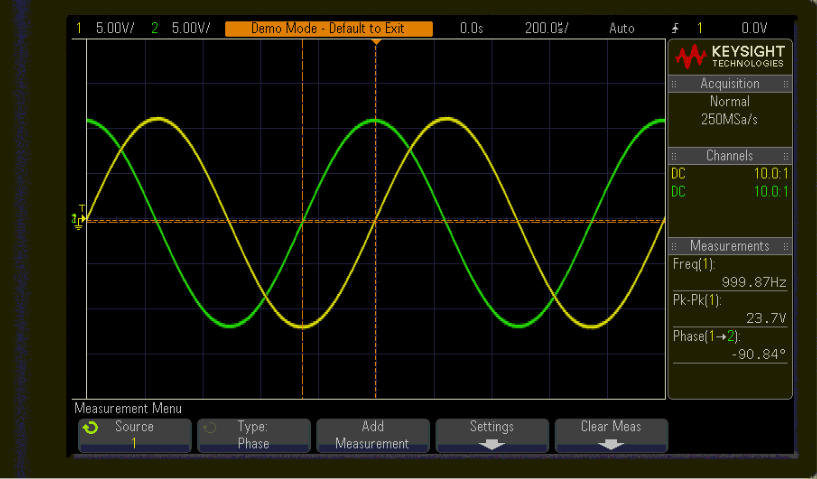
\includegraphics[width=.6\linewidth]{sinus_frek_pp_automatika.png}
\caption{Charakteristiky měřené automaticky}
\end{figure}

\begin{figure}[htbp]
	\centering
	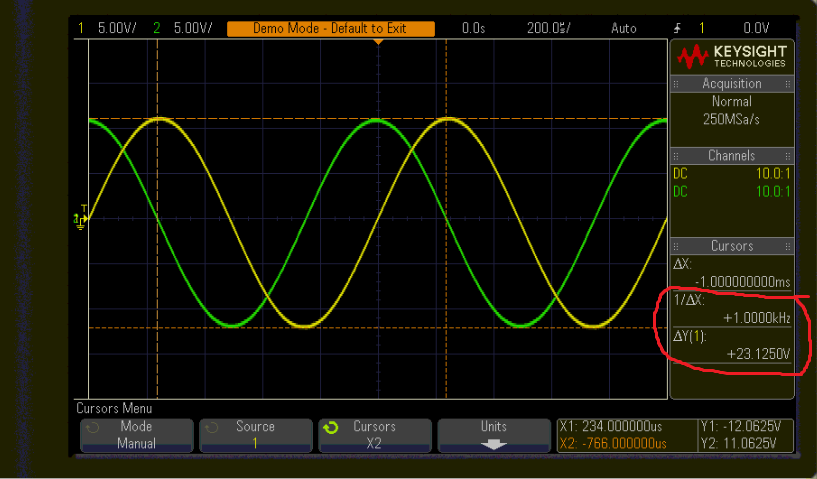
\includegraphics[width=.6\linewidth]{sinus_frek_pp_kurzor.png              }
	\caption{Charakteristiky měřené kurzorem}
\end{figure}

Automatické měření frekvence je závislé na znalosti celé periody signálu, pročež je nezbytné trochu zvětšit časovou základnu,
zatímco člověk může "tipnout" hodnotu frekvence, ačkoli vidí jen třeba půlperiodu. Ve všem ostatním ovšem automatika vede.
Protože jsou k dispozici pouze dva kurzory na každou osu (a víc by jich ani nebylo ovladatelných pro nepřehlednost),
nelze jednoduše naráz kurzorem měřit frekvenci signálu i jeho fáový posun.
Kdyby nebyly signály ideální, ale například by trošku fluktuovalo Vpp, je automatické měření k nezaplacení -- má aktualizovanou 
hodnotu vypočítánu dříve, než člověk vůbec zpozoruje, že kurzory nejsou na správném místě.

\subsection{XY zobrazení}
Užitečné pro sledování fázového rozdílu dvou signálů na stejné frekvenci.
Pakliže se frekvence liší, tvar obrazce se v čase mění, aby postihnl změny okamžitého fázového posunu.
\begin{figure}[htbp]
	\centering

	
	\begin{subfigure}{0.3\textwidth}
		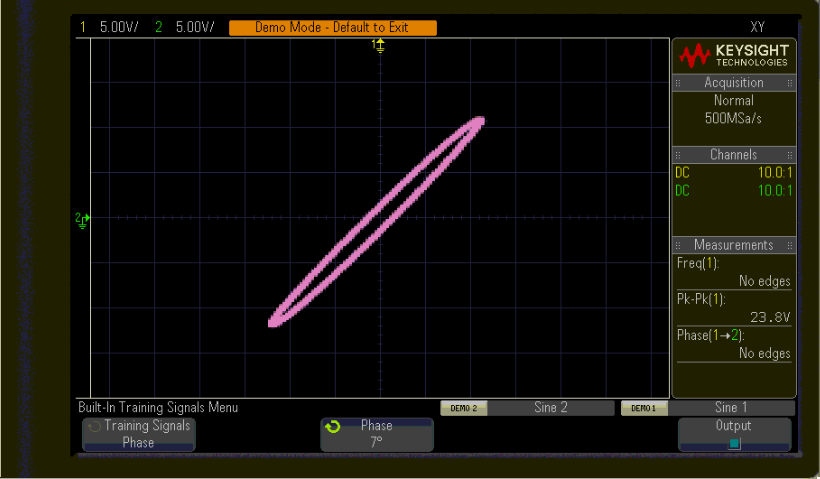
\includegraphics[width=\linewidth]{xy_7deg.png}
	\end{subfigure}
	\begin{subfigure}{0.3\textwidth}
		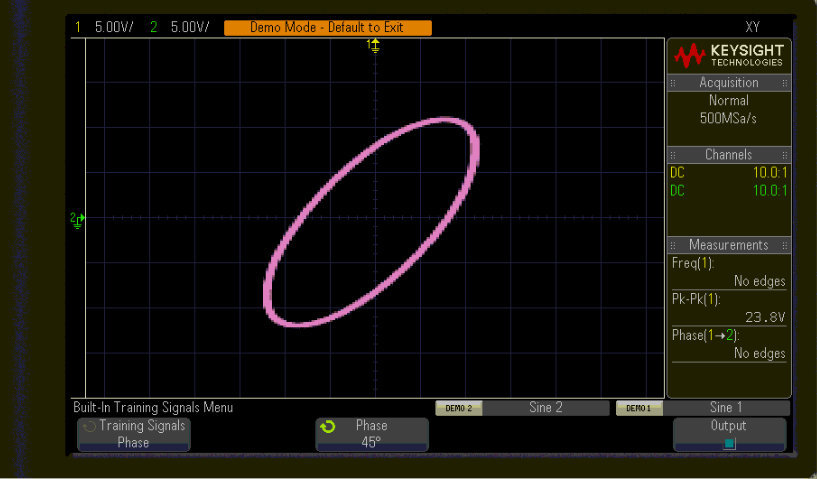
\includegraphics[width=\linewidth]{xy_45deg.png}
	\end{subfigure}
	\begin{subfigure}{0.3\textwidth}
		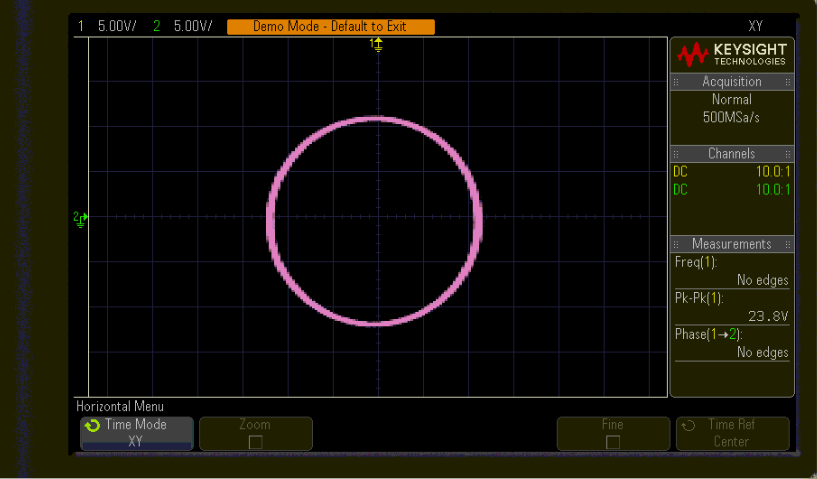
\includegraphics[width=\linewidth]{xy_90deg.png}
	\end{subfigure}
	\caption{XY zobrazení fázově posunutých signálů. Zleva doprava fázový rozdíl 7°, 45° a 90°}
\end{figure}

\subsection{Matematika}
\begin{figure}[htbp]
	\centering
	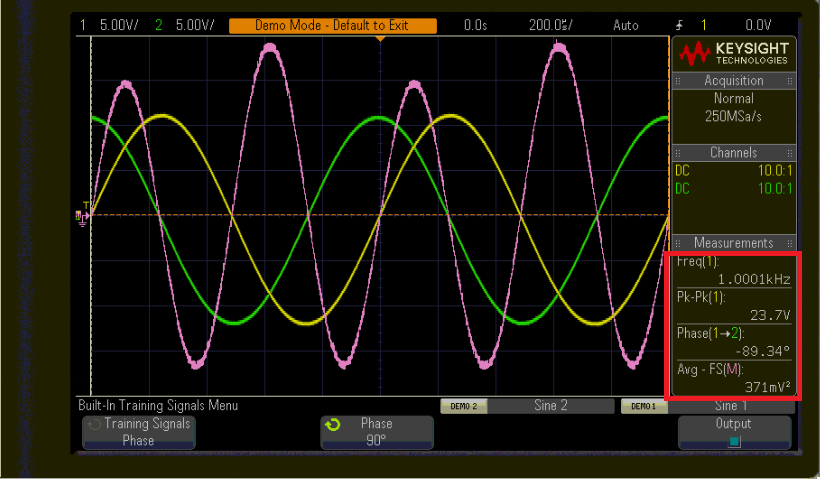
\includegraphics[width=.8\linewidth]{sinus_matematika_stredni_hodnota.png  }
	\caption{Součin dvou posunutých harmonických signálů}
	\label{fig:vykon}
\end{figure}
Pakliže by harmonické signály představovaly proud a napětí, jejich součin bude odpovídat okamžitému výkonu,
což bude harmonický signál na dvojnásobné frekvenci.
Integrací přes časový úsek (ideálně periodu) a rozkladem na složky vzniká činný a jalový výkon.
Činný výkon bude nulový na prvcích bez ohmického odporu, tedy induktoru a kapacitoru. Konkrétně v případě \ref{fig:vykon}
by mohl být kanál 1 (žlutý) napětím a kanál 2 (zelený) proudem. Poté by matematický kanál představoval výkon na kapacitoru,
jehož reálná složka je nulová kvůli fázovému rozdílu I a U o $\frac{\pi}{2}$. 


\section{Trigger}

\subsection{Auto vs normal}

Když je na vstupu osciloskopu signál a je splněna trigger condition (například signál projde přednastavenou úrovní ve směru
vzestupném/spádném, na který je osciloskop citlivý), jsou oba módy identické. Pokud ale trigger condition splněna není, poté normal mode jen sampluje a čeká
(symbol \textbf{Trig'd?} v horním pravém rohu), zatímco autotrigger čas od času pustí vzorkování a vykreslí
průběh bez ohledu na trigger condition (viz \ref{fig:trigger_mode}) Protože vzorkování není synchronizováno se signálem, jsou průběhy zachycovány v náhodných okamžicích a na displeji vzniká
barevná mlha. Alespoň je ale patrno, že je připojen vůbec nějaký signál.

\begin{figure}[htbp]
	\centering
	\begin{subfigure}{0.45\textwidth}
		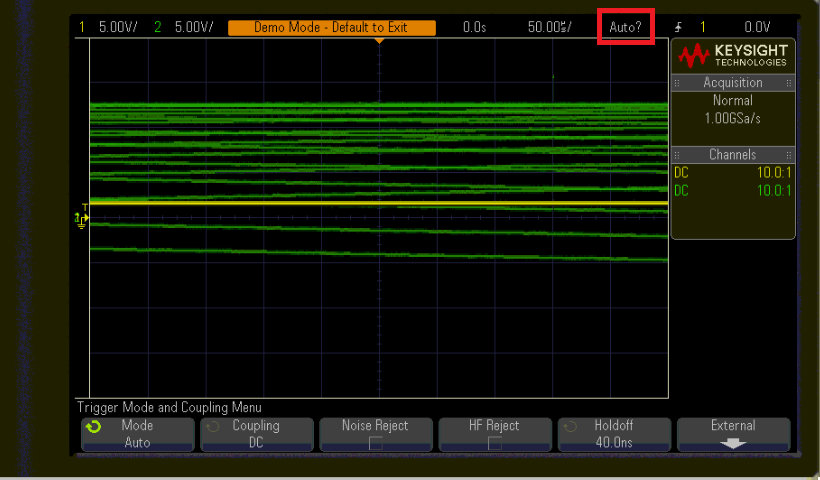
\includegraphics[width=\linewidth]{trigger_auto.png                      }
		\caption{Auto trigger (bez triggeru)}
	\end{subfigure}
	\begin{subfigure}{0.45\textwidth}
		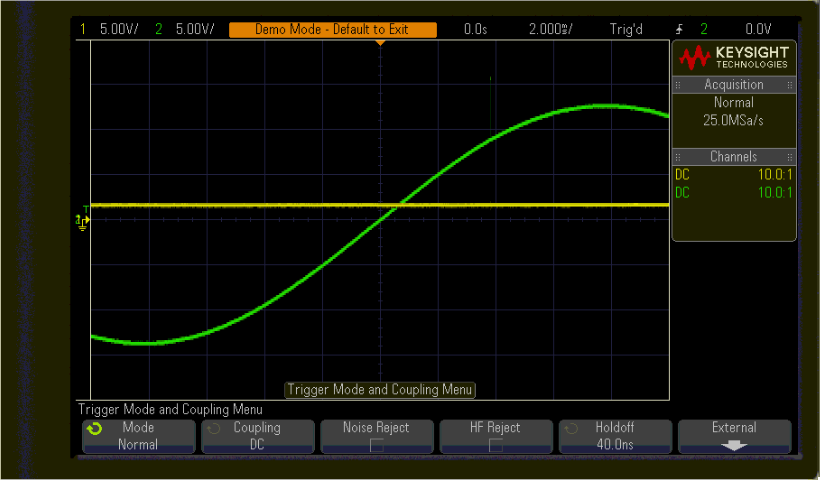
\includegraphics[width=\linewidth]{trigger_normal.png                    }
		\caption{Normal mode (trigger condition splněna)}
	\end{subfigure}
	\caption{Srovnání módů triggeru}
	\label{fig:trigger_mode}
\end{figure}

Režim auto je proto vhodný pro získání všeobecného přehledu o signálu - zda se vejde na vertikální
stupnici, zda-li se jedná o periodický děj, či jen děj přechodový atd.

\subsection{Trigger Holdoff}

Nastavení minimální prodlevy dvou po sobě jdoucích triggerů. Po detekování trigger condition začne osciloskop odpočítávat čas do reaktivace triggeru.
Nejsnazší je příklad komunikační sběrnice, po které se digitální data přenáší v \textit{rámcích}.
Průběh signálu na sběrnici lze interpretovat jako obdélník (sic s proměnlivou periodou). Kdyby byl trigger citlivý na každou hranu,
detekuje osciloskop všechny změny logické hodnoty a vykreslené průběhy se budou křížit, neboť by nastávalo více triggerů na různých místech týchž dat.
Ilustrační příklad je na obrázku \ref{fig:no_holdoff}.

Vložení nenulového pozdržení triggeru zajistí, že osciloskop počká stanovený čas a teprve následně bude hledat trigger condition.
Trigger holdoff je potřeba nastavit precizně -- nesprávný delay způsobí, že trigger bude rearmnut ještě v témže nebo až uprostřed
následujícího rámce. Obě varianty vedou na stejné problémy s křížícími se průběhy, příklad je na \ref{fig:bad_holdoff}.

\begin{figure}[htbp]
	\centering
	\begin{subfigure}{0.45\textwidth}
		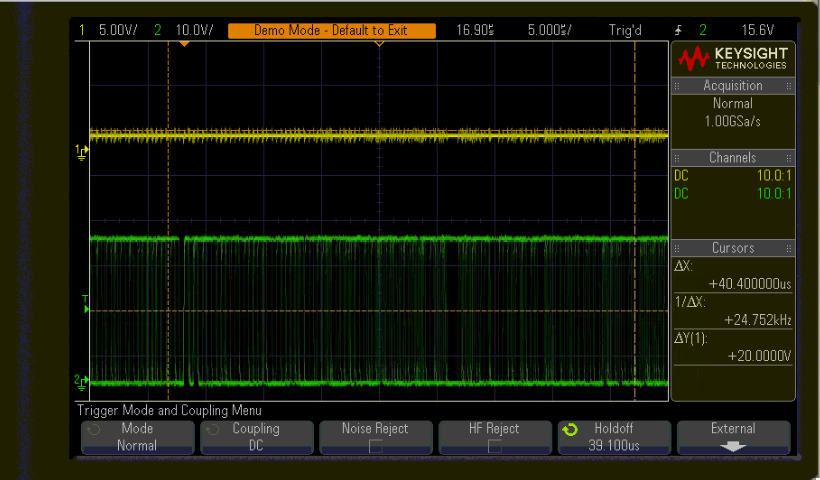
\includegraphics[width=\linewidth]{digital_glitch_bad_holdoff.png                      }
		\caption{Nesprávný holdoff, který nestačí na periodu signálu}
		\label{fig:bad_holdoff}
	\end{subfigure}
	\begin{subfigure}{0.45\textwidth}
		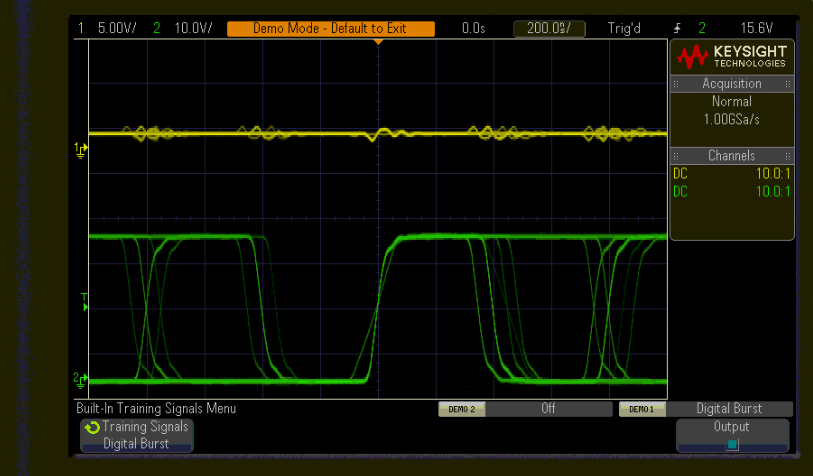
\includegraphics[width=\linewidth]{digital_glitch_no_holdoff.png                    }
		\caption{Žádný holdoff (osciloskop vnutí 40ns minimum)}
		\label{fig:no_holdoff}
	\end{subfigure}
	\caption{Nesprávná nastavení trigger holdoff}
\end{figure}

\begin{figure}[htbp]
	\centering
	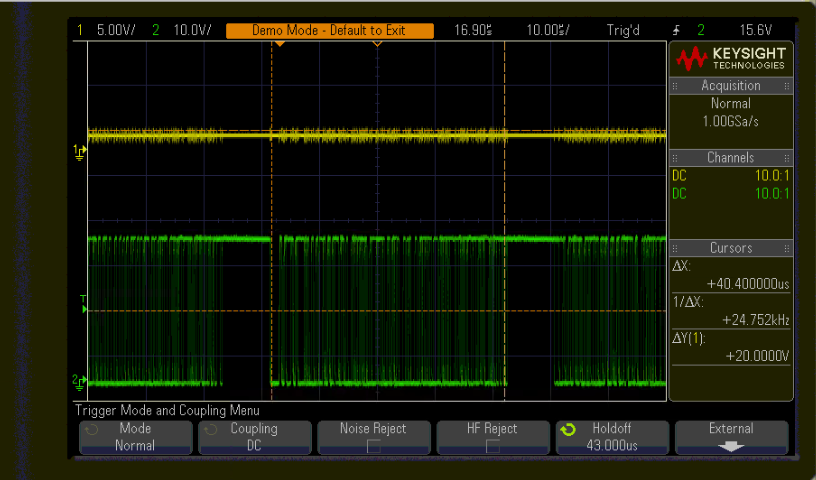
\includegraphics[width=0.8\textwidth]{digital_glitch_correct_holdoff.png                    }
	\caption{Správný holdoff na délku rámce digitálního signálu}
	\label{fig:good_holdoff}
\end{figure}
Správné nastavení pozdržení triggeru je na délku rámce, aby \textit{trigger rearm} vyšel někam doprostřed "ticha" mezi dvěma framy -- například do stop bitu na UARTu. 
Takové nastavení je vidět na obrázku \ref{fig:good_holdoff}. Protože data posílaná na simulované sběrnici jsou velice proměnlivá, pustil jsem
nejprve osciloskop v single módu. Následně jsem změnami časové základny hledal nějaké předěly, jenž by oddělovaly rámce.
Kurzory jsem identifikoval pevnou délku rámce 40 \si{\micro\second}, po které následovalo cca 8 \si{\micro\second} prodlevy.
Na obrázku je vidět, jak nastavený holdoff 43 \si{\micro\second} garantuje stabilní trigger, při kterém rámce nelítají po celé obrazovce.

\textbf{Pozn:} Pakliže jsou rámce proměnlivé délky, výrazně se situace zkomplikuje. Hodí se myšlenku trošku obrátit a třeba triggerovat
na délku pulsu větší než nějaké $T$. Tato metoda by asi nefungovala pro SPI/UART, ale fungovala by pro CAN. Standard obsahuje \textit{bit stuffing},
jehož důsledkem není možné, aby ve validním framu bylo víc jak pět stejných logických úrovní v řadě. Pakliže by data obsahovala podobný případ,
vloží se hardwarově během posílání stuffing bity, aby byl garantován dostatečný počet resynchronizačních hran v signálu.
Ve validních datech tedy nikdy nesmí být víc jak pět jedniček v řadě, zatímco \textit{End of frame} jich čítá asi sedm
(a případně ještě víc, pakliže by následně měla být sběrnice recesivní). Se znalostí baudratu lze vypočíst šířku okna recesivních úrovní
mezi rámci a trigerovat na něj.

Další uplatnění trigger holdoff je pro triggerování zarušených signálů, pro něž by se hodil třeba komparátor s hysterezí.
\begin{figure}[htbp]
	\centering
	\begin{subfigure}{0.45\textwidth}
		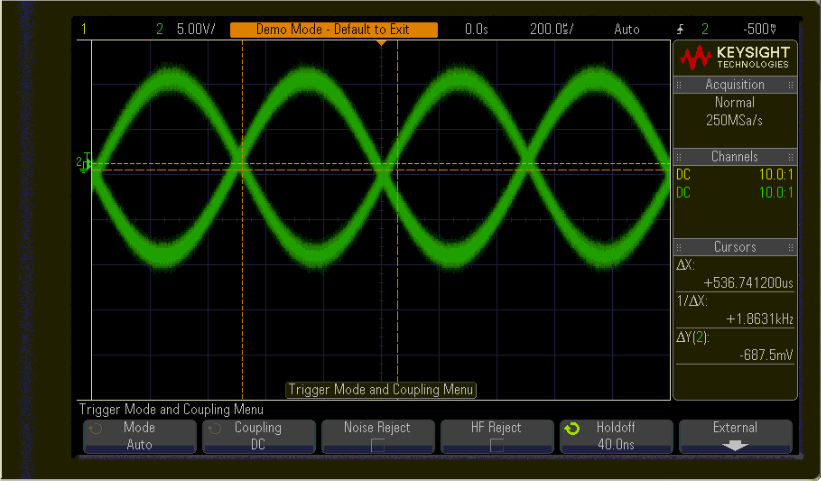
\includegraphics[width=\linewidth]{noisy_sinus_false_trigger.png                      }
		\caption{Žádný trigger holdoff -- mnoho false triggers}
		\label{fig:noisy_sin_bad}
	\end{subfigure}
	\begin{subfigure}{0.45\textwidth}
		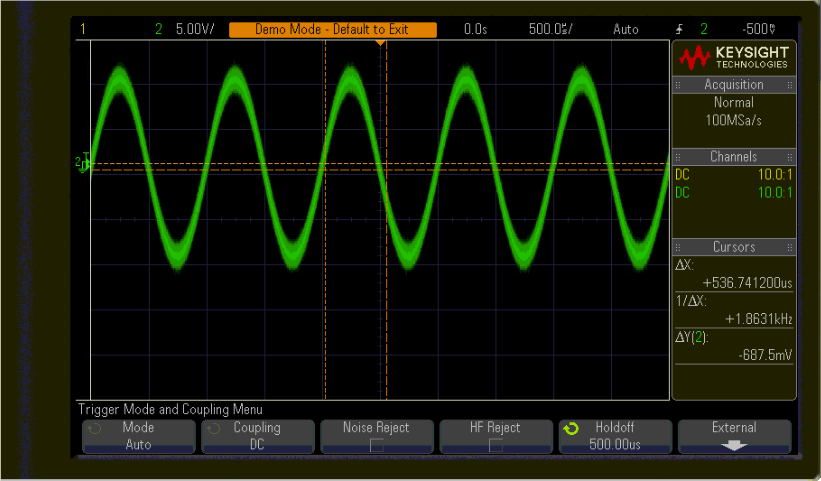
\includegraphics[width=\linewidth]{noisy_sinus_good_trigger.png                    }
		\caption{OK trigger holdoff -- ignorování šumu}
		\label{fig:noisy_sin_good}
	\end{subfigure}
	\caption{Vliv pozdržení triggeru na zarušený signál}
\end{figure}
Protože je na "hlavním signálu" superponovaný šum, nastává při průchodu signálu hladinou \textit{trigger level} velké množství \textit{trigger conditions}.
Z tohoto důvodu triggeruje osciloskop i při "spádné hraně" sinu -- ačkoli sinus samotný ryze klesá,
šum způsobuje lokální vzestupné hrany vedoucí na trigger patrný na \ref{fig:noisy_sin_bad}. Na obrázku \ref{fig:noisy_sin_good} je již nastaven 
holdoff polovina periody. Toto samo by bylo špatné nastavení, ale s ohledem na umístění triggeru nad hladinu střední hodnoty je dostatečné,
protože signál v oblasti nad triggerem stráví kratší dobu než 500 \si{\micro\second} a holdoff tak zajistí, že sestupná
hrana netrigne.



\section{Jednorázové děje}
\begin{figure}[htbp]
	\centering
	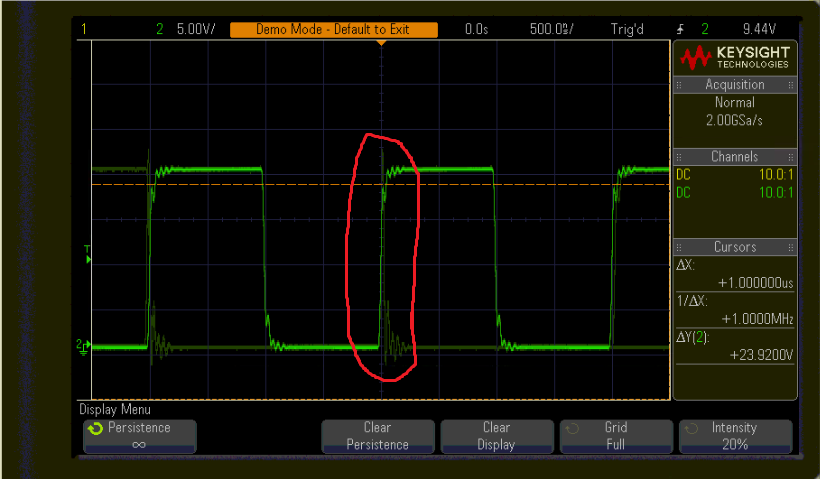
\includegraphics[width=0.8\linewidth]{clock_glitch_persistence.png                    }
	\caption{Chyba hodinového signálu zobrazená pomocí persistence}
	\label{fig:glich_persistence}
\end{figure}
Na obrázku \ref{fig:glich_persistence} je vykreslen průběh hodinového signálu se zapnutou \textit{persistence} -
dříve zobrazené průběhy se nepřepisují a zůstávají vidět, ačkoli se na obrazovku vykreslují i nové zachycené.
Pakliže je signál skutečně ideálně periodický, poté budou všechny průběhy dokonale splývat a na displeji bude zobrazena jen jedna tlustá čára.
Na obrázku je ale patrná ještě další slabá světle zelená stopa. Jedná se o relikt chyby v signálu, jež nastane třeba jednou za tisíce i miliony
period a není tak v lidských silách ji hledat ručně. Persistence nám zajistí, že i takto ojedinělý signál bude zachycen.

Stejnou chybu je možné detekovat hledáním nesprávné délky puslu v signálu a nebo aktivací \textit{runt triggeru} (viz obrázek \ref{fig:glitch_runt}).
Zde osciloskop detekuje jen pár ns široký kladný puls, který je jistě chybou, neboť šířka pulsů hodin je v řádu mikrosekund.
Frekvenční oblast takovéto chyby je pro zajímavost vykreslena na obrázku \ref{fig:fft_clock_glitch}.

\begin{figure}[htbp]
	\centering
	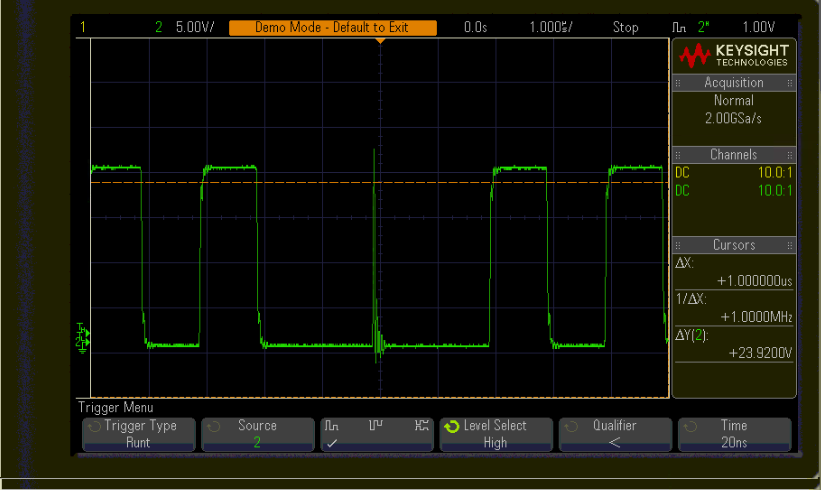
\includegraphics[width=0.8\linewidth]{trigger_runt_clock_glitch.png                    }
	\caption{Identifikace chyby hodin pomocí runt triggeru}
	\label{fig:glitch_runt}
\end{figure}

Stejná identifikace by se dala provést triggerováním na šířku pulzu a hledáním menší či naopak vyšší hodnoty. Na obrázku \ref{fig:pos_width}
je zachycen výstup mého experimentu. Osciloskop úspěšně triggeruje (viz \textit{Trig'd} v levém horním rohu obrazovky) na kladný pulz užší než 540 ns.
Ovšem kvůli nesprávně nastavenému posunu na časové ose není glitch vidět, protože je mimo obrazovku... Pro srovnání vedle na obrázku \ref{fig:neg_width} je patrno,
že osciloskop není schopen nalézt trigger condition na krátký záporný puls.

\begin{figure}[htbp]
	\centering
	\begin{subfigure}{0.45\textwidth}
		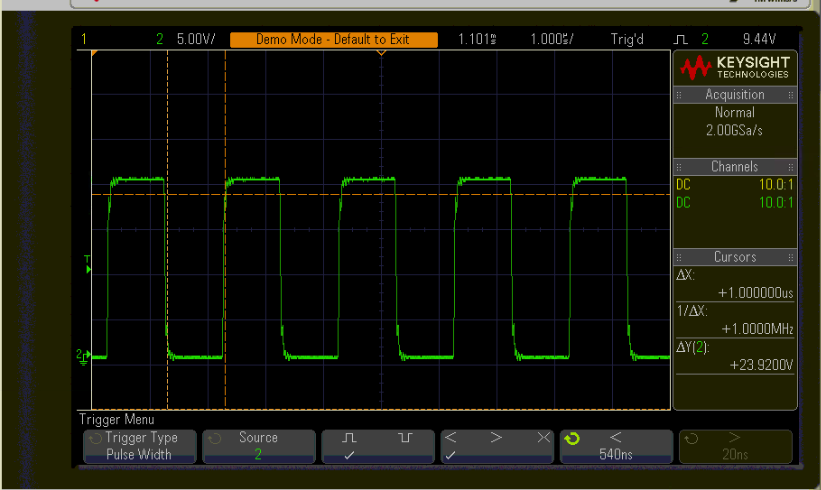
\includegraphics[width=\linewidth]{trigger_pulsewidth_pos_trigged_wut.png                      }
		\caption{Trigger na malou šířku kladného pulzu}
		\label{fig:pos_width}
	\end{subfigure}
	\begin{subfigure}{0.45\textwidth}
		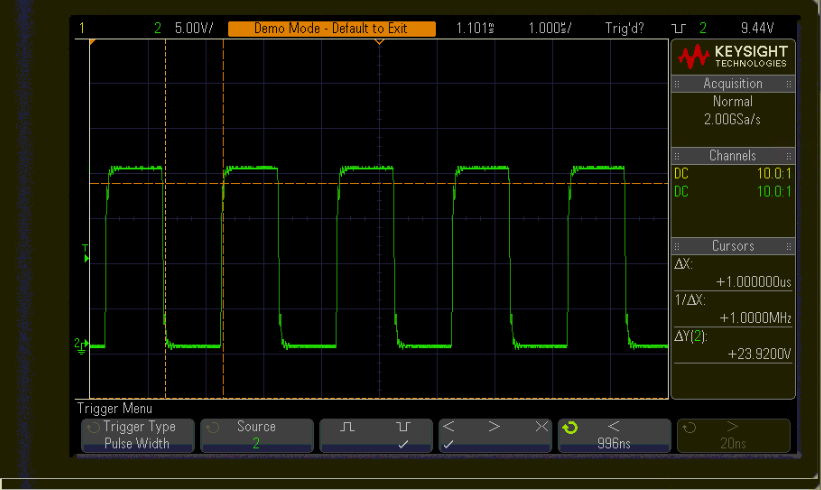
\includegraphics[width=\linewidth]{trigger_pulsewidth_never.png                    }
		\caption{Bez triggeru na malou šířku záporného pulzu}
		\label{fig:neg_width}
	\end{subfigure}
	\caption{Hledání glitche pomocí triggeru nastaveného na malou šířku pulsu}
\end{figure}

Toto souhlasí s časovým průběhem chyby podle obrázku \ref{fig:glitch_runt}.
Všechny zdravé pulsy jsou široké 1 \si{\micro\second}. Při chybě nastane dlouhá nula, krátký kladný puls, opět dlouhá nula a následují zdravé pulzy.
Nikde není obsažen záporný pulz. Abychom triggerovali na něj, bylo by nejspíše potřeba umístit trigger level kamsi na úroveň zákmitů bezprostředně po kladném pulzu.
Podle této logiky by mělo být možné triggerovat na dlouhý záporný puls, neboť ta "dlouhá nula před pulsem" zmiňovaná výše je v principu záporným pulsem.
Obrázek \ref{fig:neg_width_trigger} sice rovněž trpí mojí chybou se špatnou pozicí na časové ose, potvrzuje ovšem domněnku, že lze triggernout na dlouhý záporný puls.

\begin{figure}[htbp]
	\centering

	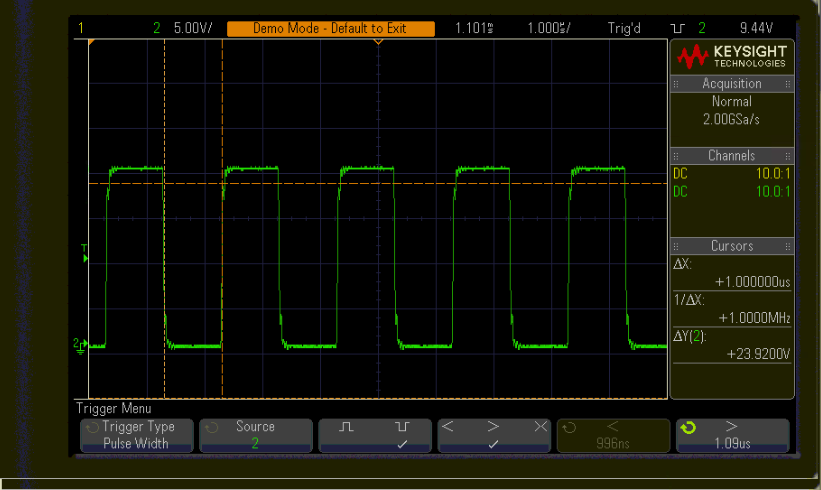
\includegraphics[width=0.8\linewidth]{trigger_pulsewidth_neg_triggers_always_wut.png         }
	\caption{Trigger na dlouhý záporný puls}
	\label{fig:neg_width_trigger}
\end{figure}	

\section{Vzorkování}

Na obrázku \ref{fig:rf_20ms} je vidět zelený mrak divokého (a na první pohled člověk tuší, že asi i podvzorkovaného) RF signálu. Osciloskop oznamuje,
že pro danou časovou základnu 2ms vzorkuje frekvencí $f_s$ = 50 MSa/s, čemuž odpovídá vzorkovací krok $h_s$ = 20ns. Protože osciloskop je schopen signál přiblížit
na takovou časovou základnu, je možné se podívat přímo na jednotlivé vzorky, jak byly osciloskopem zachytávány. Obrázek \ref{fig:rf_20ns} ukazuje jednotlivé vzorky
(zlomy časového průběhu) zarovnané na dílky časové základny. Kmitočet vzorkování není dostatečný.

\begin{figure}[htbp]
	\centering
	\begin{subfigure}{0.45\textwidth}
		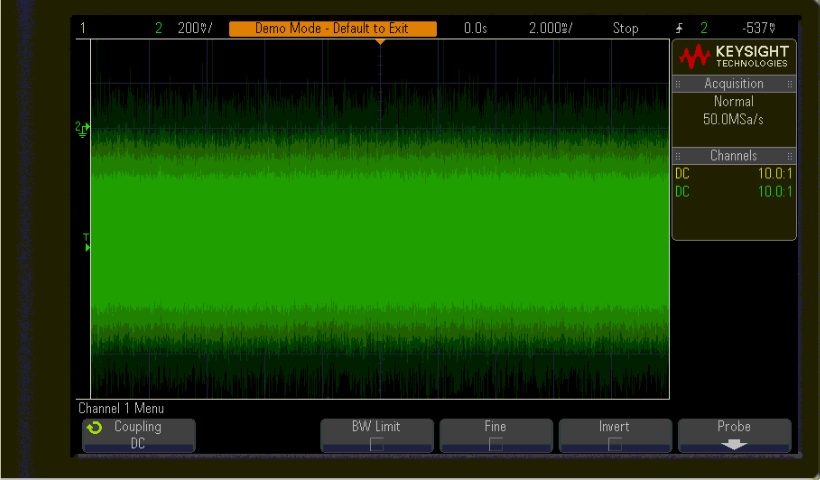
\includegraphics[width=\linewidth]{rf_captured20ms_view20ms.png                      }
		\caption{RF signál s časovou základnou 2 ms}
		\label{fig:rf_20ms}
	\end{subfigure}
	\begin{subfigure}{0.45\textwidth}
		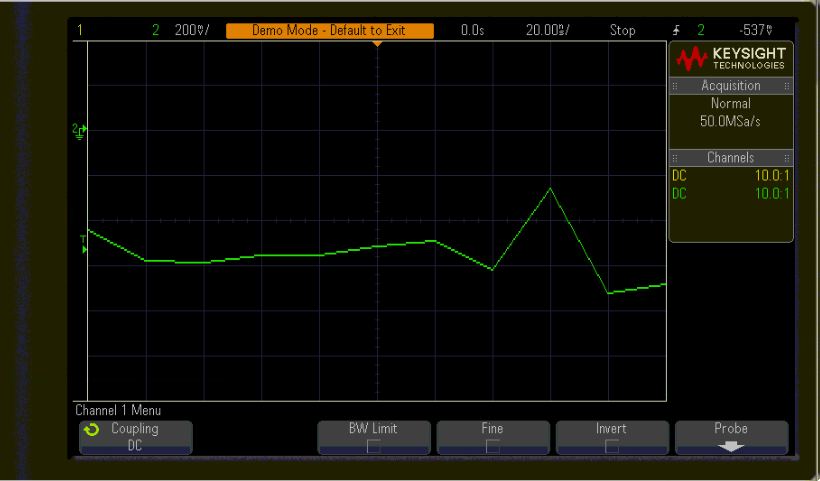
\includegraphics[width=\linewidth]{rf_captured20ms_view20ns.png                    }
		\caption{RF signál s časovou základnou 20 ns}
		\label{fig:rf_20ns}
	\end{subfigure}
	\caption{Vysokofrekvenční signál osekaný konečnou vzorkovací frekvencí}
\end{figure}

Obrázky \ref{fig:rf_50us} a \ref{fig:rf_5ns} napravují tento nedostatek. Zvolením nižší časové základny pouhých 50 \si{\micro\second}
se zdánlivě nic moc nezmění při pohledu z dálky (obrázek \ref{fig:rf_50us}), ovšem díky čtyřicetkrát vyšší vzorkovací frekvenci 2 GSa/s
není ani při maximálním podporovaném přiblížení na časovou základnu 5ns možné pozorovat ostré zuby způsobené vzorkováním (chyba
způsobená vzorkovacím krokem se ztratí ve srovnání s kvantizační chybou převodu analogového signálu AD převodníkem a chybou rozlišení
obrazovky). 

\begin{figure}[htbp]
	\centering
	\begin{subfigure}{0.45\textwidth}
		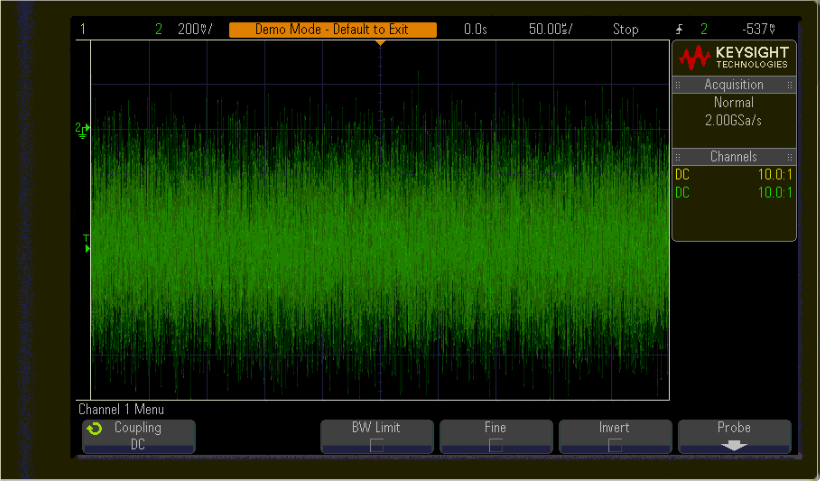
\includegraphics[width=\linewidth]{rf_captured50us_view50us.png                 }
		\caption{RF signál s časovou základnou 50 \si{\micro\second}}
		\label{fig:rf_50us}
	\end{subfigure}
	\begin{subfigure}{0.45\textwidth}
		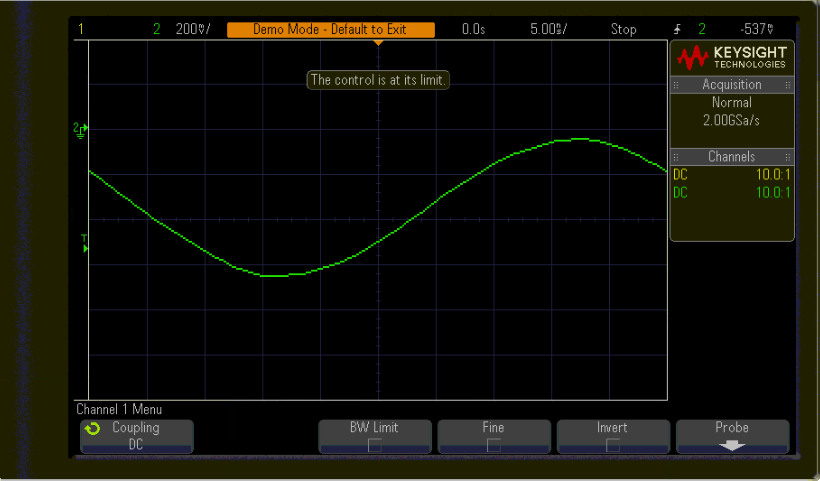
\includegraphics[width=\linewidth]{rf_captured50us_view5ns.png                    }
		\caption{RF signál s časovou základnou 5 ns}
		\label{fig:rf_5ns}
	\end{subfigure}
	\caption{Zanedbatelnost chyby způsobené konečností vzorkovací frekvence}
\end{figure}

\section{Fourierova transformace}

\begin{figure}[htbp]
	\centering
	\begin{subfigure}{0.45\textwidth}
		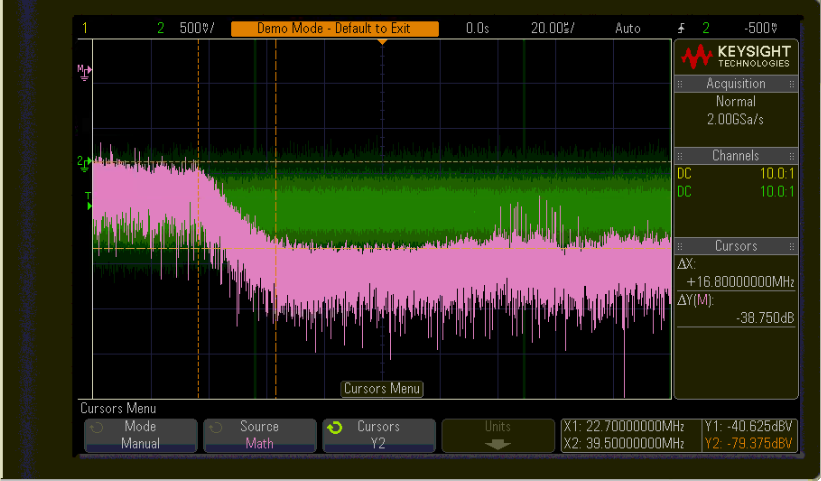
\includegraphics[width=\linewidth]{rf_fft_amplitudy.png         }
		\caption{Významné hodnoty transformace}
		\label{fig:fft_rf}
		\end{subfigure}
	\begin{subfigure}{0.45\textwidth}
		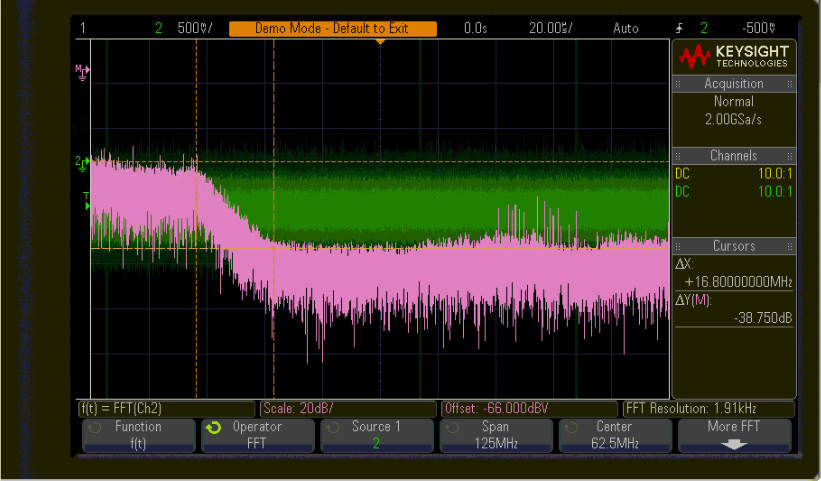
\includegraphics[width=\linewidth]{rf_fft_resolution.png                    }
		\caption{Použité nastavení transformace}
		\label{fig:fft_rf_config}
	\end{subfigure}
	\caption{Fourierka RF signálu na plném rozsahu}
\end{figure}

Navazuji prací s RF signálem z minulé úlohy. Analýzou signálu na \ref{fig:rf_5ns} se dá velmi hrubě odhadnout, že RF signál obsahuje i frekvenci 20 MHz.
Podle toho je jasné, že bude potřeba mít velký rozsah FFT (protože osciloskop fixuje počet vzorků pro výpočet FFT, je velký rozsah spojen s malým rozlišením (= velkým krokem)
ve frekvenční oblasti). Pro začátek tedy nastavme FFT na rozsah cca 100 MHz. Výstup je zachycen na obrázku \ref{fig:fft_rf} a konfigurace FFT na obrázku \ref{fig:fft_rf_config}.
Pomocí kurzorů jsou vyznačeny dvě části spektra.
Terminologií teorie signálů se dá hovořit o (alespoň ve srovnání se zbytkem) propustné části pro frekvence od DC až po 22 MHz,
nepropustné (zatlumené) části od frekvence 40 MHz dál a pásmu přechodu na intervalu frekvencí $f \in \left[ 22, 40 \right]$ MHz, kde nastává pokles amplitud o 40db na oktávu.


Odhadněme, že bandwidth systému generujícího tento signál je 22 MHz. Vysoké frekvence jsou stoprocentně pouze šumy. Na obrázku \ref{fig:fft_bandwidth}
je vykreslena fourierka téhož signálu, ovšem s upraveným nastavením - omezením se na menší rozsah frekvencí při zachování počtu vzorků se dosáhne lepšího rozlišení 
(menšího kroku) transformace. Je vidět, že žádná frekvence výrazně nedominuje, RF signál tak lze považovat za bílý šum. 

\begin{figure}[htbp]
	\centering

	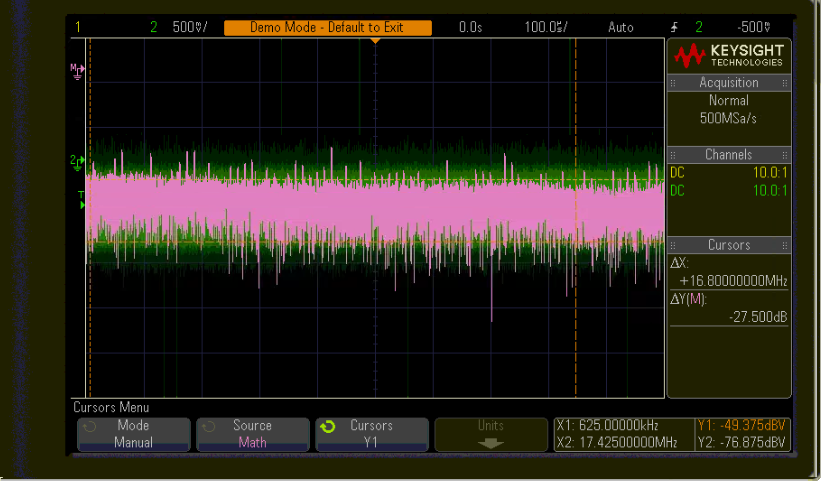
\includegraphics[width=0.8\linewidth]{rf_fft_bandwidth.png         }
	\caption{Fourierka RF signálu na menším rozsahu}
	\label{fig:fft_bandwidth}
\end{figure}	



Zajímavá je frekvenční oblast signálu z obrázku \ref{fig:noisy_sin_good} vykreslená na obrázku \ref{fig:fft_noisy}.
Jedná se o sinus s amplitudou řádově 10V na frekvenci 1kHz zarušený vysokofrekvenčním šumem.
Na výstupu FFT je skutečně vidět jeden peak na frekvenci 1kHz s amplitudou 17 dB (+20 dB v amplitudě odpovídá 10 jednotkám v lineární stupnici, takže toto měření velmi obstojně
souhlasí s očekáváním), zatímco zbytek spektra je naplněn šumem s amplitudou -40dB.

\begin{figure}[htbp]
	\centering
	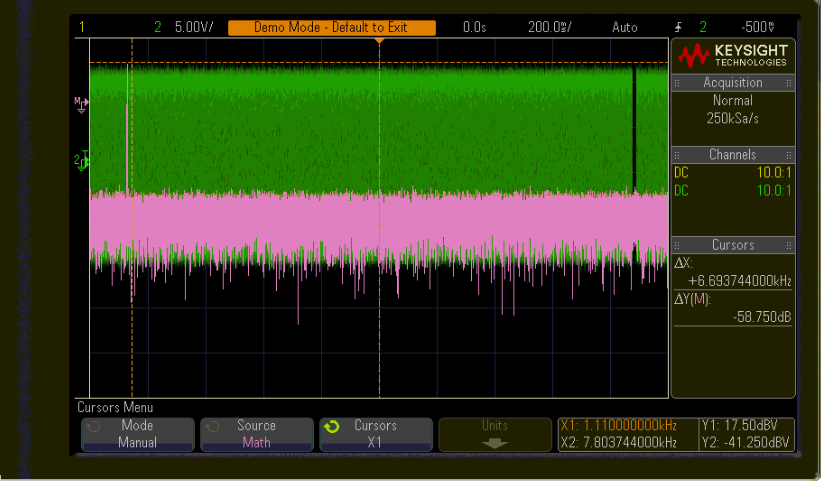
\includegraphics[width=0.8\linewidth]{noisy_sinus_fft.png         }
	\caption{Frekvenční spektrum zarušeného sinu}
	\label{fig:fft_noisy}
\end{figure}	



V úloze výše byl analyzován hodinový signál na 500 kHz s občasným glitchem. Pro zajímavost je přiloženo jeho frekvenční spektrum na obrázku \ref{fig:fft_clock_glitch}.
V levé části je vidět standardní fourierka obdélníkového signálu sestávající z lichých harmonických, která s rostoucím indexem harmonické odeznívá amplitudou do nuly.
Výrazně dál ve spektru je druhý peak příslušící nejspíše k rychlým hranám glitche.
\begin{figure}[htbp]
	\centering
	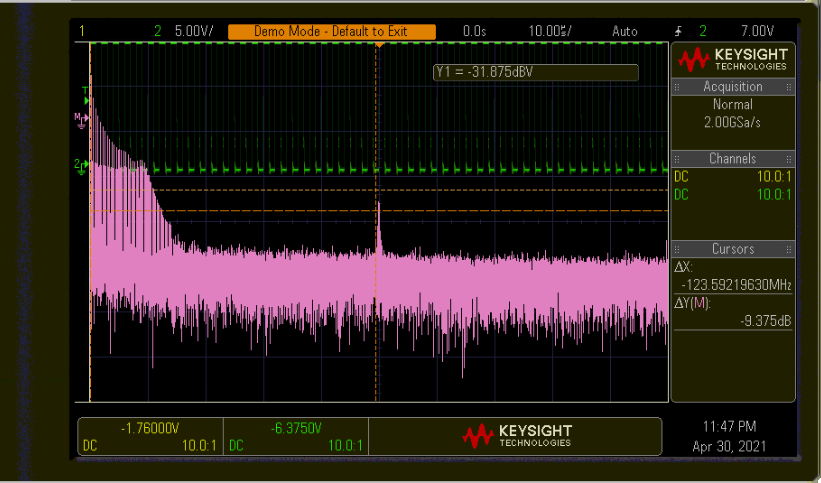
\includegraphics[width=0.8\linewidth]{clock_glitch_fft.png                    }
	\caption{Chyba hodin ve frekvenční oblasti }
	\label{fig:fft_clock_glitch}
\end{figure}

		\begin{thebibliography}{9}
			
			
			\bibitem{zadani}
			Tým vyučujících SME, Zadání úlohy na Moodle, \url{https://moodle.fel.cvut.cz/pluginfile.php/296878/mod_resource/content/1/advanced_remote_scope_v2.pdf}
			
			\bibitem{rickroll}
			Keysight academy: Oscilloscope mastery in less than five years, \url{https://www.youtube.com/watch?v=dQw4w9WgXcQ}
			
			\bibitem{motivace}
			Motivační hudba, \emph{Kirby dream land theme song} \url{https://www.youtube.com/watch?v=3CS93CdMv_E}
			
		\end{thebibliography}
		
		\end{document}
		
		